\documentclass[t]{beamer}
\usepackage{CJKutf8}
\usepackage{amsfonts}
    \usepackage{amsmath}
    \usepackage{amssymb}
    \usepackage{amsthm}
    \usepackage{enumerate}
    \usepackage{graphicx}
    \usepackage{layout}
    \usepackage{mathrsfs}
    \usepackage{fancyhdr}
    \usepackage{subfigure}
    \usepackage{tcolorbox}
    \usepackage{tikz-cd}
    \usepackage{color}
    \usepackage{pifont}
    \usepackage{verbatim}
    \usepackage{mathtools}
    \usepackage{float}
    \usepackage{bm}
    \usetheme{AnnArbor}
% \usetheme{Antibes}
\usecolortheme{beaver}
\usepackage{listings}

% 设置JSON样式
\lstdefinestyle{json}{
    basicstyle=\tiny\ttfamily,
    columns=fullflexible,
    showstringspaces=false,
    commentstyle=\color{gray},
    keywordstyle=\color{blue},
    stringstyle=\color{red},
    breaklines=true,
    frame=single,
    captionpos=b,
    aboveskip=10pt,
    belowskip=10pt
}

\lstset{
    language=Python, % 设置代码块语言为Python
    breaklines=true, % 自动换行
    basicstyle=\small\ttfamily, % 设置基本字体样式
    keywordstyle=\bfseries\color{blue}, % 设置关键字样式
    commentstyle=\itshape\color{gray}, % 设置注释样式
    showstringspaces=false, % 不显示字符串中的空格
    frame=single, % 设置代码块边框样式
    numbers=left, % 行号显示在左侧
    numberstyle=\tiny\color{gray}, % 设置行号样式
    stepnumber=1, % 设置行号间隔
    tabsize=4 % 设置制表符宽度
}


% 设置shell样式
\lstdefinestyle{shell}{
    language=bash,
    basicstyle=\tiny\ttfamily,
    columns=fullflexible,
    showstringspaces=false,
    commentstyle=\color{gray},
    keywordstyle=\color{blue},
    stringstyle=\color{red},
    breaklines=true,
    frame=single,
    captionpos=b,
    aboveskip=10pt,
    belowskip=10pt
}

% 添加网址的命令
\usepackage{hyperref}
% 这是一个带链接文本的示例:\href{https://www.example.com}{点击这里访问网站}
% 普通的示例:\url{https://www.example.com}
% 表格
\usepackage{booktabs}
\usepackage{multirow}

% \setbeamertemplate{navigation symbols}{}

\usepackage{textpos}

\newcommand{\dif}{\mathrm{d}}
\newtheorem{thm}{{定理}}

% some common command
\newcommand{\mm}[1]{$ #1$\newline}
% \newcommand{\tuichu}{\Rightarrow}
% \newcommand{\li}[1]{\newline#1}



\newcommand{\analysis}[2]{\forall \mathcal{E}{#1},\exists \delta {#2},s.t.}
\newcommand{\denyanalysis}[2]{\exists \mathcal{E}{#1},\forall \delta {#2},s.t.}
\newcommand{\yield}{\Rightarrow }
\newcommand{\jj}{\newline}
\newcommand{\ff}[1]{$ #1$}   % math environment + newline
\newcommand{\fgn}[1]{\begin{equation}#1\end{equation}  }
\newcommand{\fg}[1]{$$ #1$$}   % math environment + newline 
\newcommand{\pf}{$proof.$\newline}
\newcommand{\ee}{\newline\ff{\Box}\newline}
\newcommand{\fenshi}[2]{\ff{\frac{#1}{#2}}}
\newcommand{\shenlue}{\vdots\jj}
\newcommand{\abs}[1]{{\left \lvert #1 \right\rvert}}
\newcommand{\loge}[1]{In ({#1})}
\newcommand{\logical}[2]{log_{#2}^{#1}}
\newcommand{\summary}[3]{$\sum_{{#1}={#2}}^{#3}  $}
\newcommand{\denjia}[2]{{#1}\Leftrightarrow {#2}}
\newcommand{\jihe}[3]{ {#1}  = \{ {#2} \mid {#3} \} }
\newcommand{\ve}[2]{\left\langle {#1},{#2}\right \rangle}
\newcommand{\dakuohao}[2]{\begin{array}{rcl}{#1}\end{array} \} \Rightarrow{#2}}
\newcommand{\sxb}[3]{#1^{#2}_{#3}}
\newcommand{\sss}[2]{#1^{#2}}
\newcommand{\xxx}[2]{#1_{#2}}
\newcommand{\bri}[1]{\uppercase\expandafter{\romannumeral#1}}
\newcommand{\ri}[1]{\romannumeral#1} 
\newcommand{\polynomial}[8]{#1_{#2}#6^{#7}+#1_{#3}#6^{#8}+...+#1_{#4}#6+#1_{#5} }
\newcommand{\newd}[4]{f[{#1}_{#2},{#4},{#1}_{#3}]}
\newcommand{\lb}[2]{\begin{align*}\begin{split}{#1}\{ {#2}\end{split}\end{align*}}
\newcommand{\tab}[1]{\begin{array}{ll} {#1}\end{array}}


% 向量乘积
\newcommand{\avg}[1]{\left\langle #1 \right\rangle}
% 偏微分方程
\newcommand{\difFrac}[2]{\frac{\dif #1}{\dif #2}}
\newcommand{\pdfrac}[2]{\frac{\partial{#1}}{\partial{#2}}}
% 不同章节
\newcommand{\one}[1]{\section{#1}}
\newcommand{\two}[1]{\subsection{#1}}
\newcommand{\three}[1]{\subsubsection{#1}}
\newcommand{\aone}[1]{\section*{#1}}
\newcommand{\atwo}[1]{\subsection*{#1}}
\newcommand{\athree}[1]{\subsubsection*{#1}}
% 大括号,左右都有
\newcommand{\lbra}[1]{\left\{  {\begin{matrix} #1 \end{matrix}}\right. } 
% 样式 括号前缀 + 括号 
\newcommand{\lbras}[2]{{#1}\left\{ {  {\begin{matrix} #2 \end{matrix}}}\right. } 
\newcommand{\rbra}[1]{ \left.  {\begin{matrix} #1 \end{matrix}} \right\}  } 
% 模长
\newcommand{\distance}[1]{\parallel #1\parallel }
% 等价
\newcommand{\equ}{\Longleftrightarrow }
% 共轭
\newcommand{\cja}[1]{\overline{#1}}
% 两个矩阵,上面是 方框[] 下面是线条| 中间是 无
\newcommand{\mtx}[1]{\begin{matrix}#1\end{matrix} }
\newcommand{\bmtx}[1]{\begin{bmatrix}#1\end{bmatrix} }
\newcommand{\vmtx}[1]{\begin{vmatrix}#1\end{vmatrix} }
% \newcommand{\table}[1]{\begin{array}[lr]{ccc} #1 \end{array}}

%输入普通字符
\newcommand{\ww}[1]{\text{#1}}

% 所有内容 直接头文件搞定
\newcommand{\everything}[1]{\begin{document}\begin{CJK*}{UTF8}{gkai}#1\end{CJK*}\end{document}}


% 存放代码(失败了)
\newcommand{\cccode}[1]{\begin{lstlisting}#1\end{lstlisting}}

% 改变特定行序列
\newcommand{\ttt}{\subsection{}}

% 嵌套序号
\newcommand{\eee}[1]{\begin{enumerate}#1\end{enumerate}}


% 模板里面的一些宏
\newcommand{\pdfFrac}[2]{\frac{\partial #1}{\partial #2}}
\newcommand{\OFL}{\mathrm{OFL}}
\newcommand{\UFL}{\mathrm{UFL}}
\newcommand{\fl}{\mathrm{fl}}
\newcommand{\op}{\odot}
\newcommand{\Eabs}{E_{\mathrm{abs}}}
\newcommand{\Erel}{E_{\mathrm{rel}}}
% 变化颜色
\newcommand{\red}{\textcolor{red}}
\newcommand{\blue}{\textcolor{blue}}
% 注释代码
% \newcommand{\undef}[1]{\iffalse #1 \fi}

% 流程图需要用到的宏包
\usepackage{palatino}
\usepackage{tikz}
\usetikzlibrary{shapes.geometric, arrows}
\tikzstyle{startstop} = [rectangle, rounded corners, minimum width = 2cm, minimum height=1cm,text centered, draw = black, fill = red!40]
\tikzstyle{io} = [trapezium, trapezium left angle=70, trapezium right angle=110, minimum width=2cm, minimum height=1cm, text centered, draw=black, fill = blue!40]
\tikzstyle{process} = [rectangle, minimum width=3cm, minimum height=1cm, text centered, draw=black, fill = yellow!50]
\tikzstyle{decision} = [diamond, aspect = 3, text centered, draw=black, fill = green!30]
% 箭头形式
\tikzstyle{arrow} = [->,>=stealth]
% 4个非常重要 的新命令
\newcommand{\start}[2]{    \node (start) [startstop]{#1};\node (in1) [io, below of = start]{#2};\lin{start}{in1}{}}
\newcommand{\stopp}[3]{\node (out1) [io, below of= #1]{#2};\node (stop) [startstop, below of=out1]{#3};\lin{out1}{stop}{} }
\newcommand{\pro}[6]{    \node (#3) [process, #2 of=#1,xshift=#4 cm]{#5};}
\newpage
\newcommand{\lin}[3]{\draw [arrow] (#1) --node [above] {#3} (#2);}


\begin{document}
\begin{CJK*}{UTF8}{gkai}
% 一般第一页显示PPT标题以及作者信息

% \BackgroundPic{./Screenshot from 2022-04-20 16-31-08.png}

% 增加学校 前面
\addtobeamertemplate{title page}{}{
	\begin{tikzpicture}[remember picture,overlay]
		% \node[yshift=85pt,xshift=50pt]{\includegraphics[height=2cm]{Screenshot from 2022-04-20 16-51-21.png}};
\end{tikzpicture}
}


	% \title{时间序列数据集}
	\title{组会汇报}
	\subtitle {} %不需要
	\author{
		陈钶杰\, \\
		专业:计算数学\,
	} % 显示作者
	% \institute {学院:数学科学学院} % 设置学院机构	
	\date{\today}  % 显示日期
\titlepage

% 设置目录
\begin{frame}{目录}
\frametitle{目录}	
\tableofcontents  % 显示目录
\end{frame} 


\section{论文阅读:}

\subsection{思维之树}
\begin{frame}
    \frametitle{问题背景}
    % 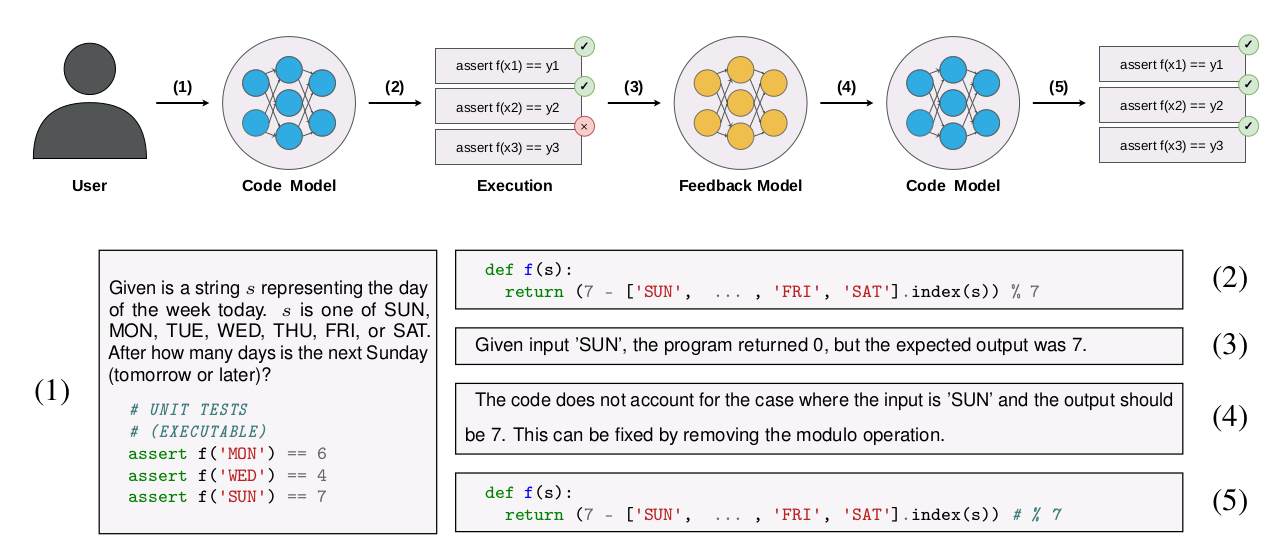
\includegraphics[scale=0.25]{png/example.png}
    \begin{itemize}
        \item 大模型的推理过程是一个token级别的,从左到右的一个决策过程,对比人类的思考方式来说,有着非常大的局限(例如人类写文章,写着写着发现写错了,我们可以回过头来,重新修改前面的内容,然后再继续往后写,而大模型LM不能这样),这使得大模型在需要探索,全局分析(前瞻探索或者回溯),初步决策发挥关键作用的任务中效果不太好。
        \item 即现有的大模型有如下的缺点:
        \eee{
            \item 局部性:现有LM模型不会在思维过程中探索不同的延续,即不会去探索当前节点的其他分支解决方案。
            \item 缺乏全局性:大模型LM没有纳入任何类型的规划、展望或回溯来帮助评估不同的选项。
        }
        \item 人类推理特点:可以重复使用可用的信息来进行启发式的探索,促使挖掘出更多真正有用的信息,找到最终的解决方案。
    \end{itemize}
\end{frame}

\begin{frame}
    \frametitle{Tree of Thoughts方法}
    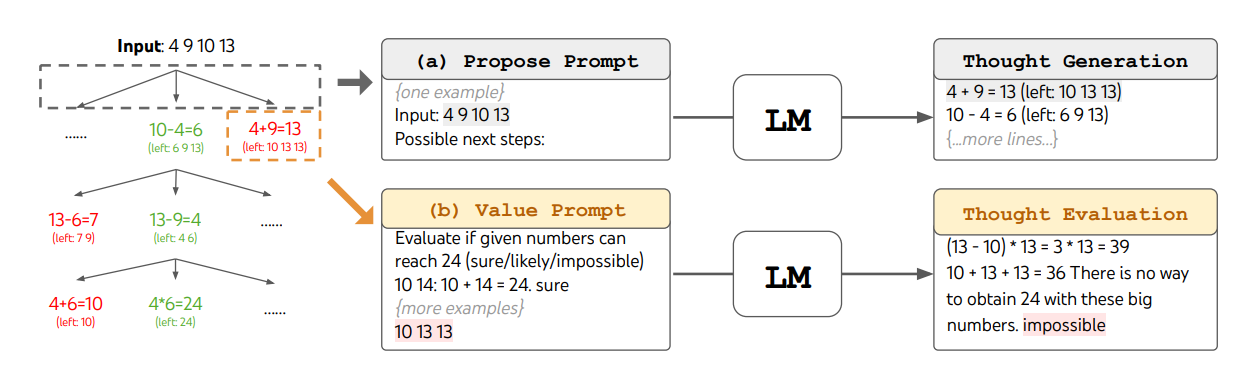
\includegraphics[scale=0.28]{png/process.png}
    \begin{itemize}
        % \item 提出了Tree of Thoughts(ToT)方法:其允许LM通过考虑多种不同的推理路径并且能进行自我评估选择来决定下一步行动,并在必要时looking ahead或回溯以做出全局选择(可以用dfs或者bfs等方法做全局探索),从而进行深思熟虑的决策
        % \item 主要通过Thought decomposition【thought分解】,Thought generator【thought生成】,State evaluator【状态评估】,Search algorithm【搜索算法】四个步骤完成,详情如下
        \item 用一个算24点的例子,来说明具体使用思维树.\\
        \eee{
            \item 思维分解:问题的提问方式可能一样(都是一句话),但是问题类型可以进行细分,比如算24点就是运算一行方程.
            \item 思维生成:生成多种可能,比如像上图中的多行thoughts.
            \item 思维评估:对生成的thoughts进行可能性分析.
            \item 搜索算法:选择合适的算法进行最优结果的搜索.比如这里选择BFS.
        }
    \end{itemize}
\end{frame}

\begin{frame}
    \frametitle{总结}
    % 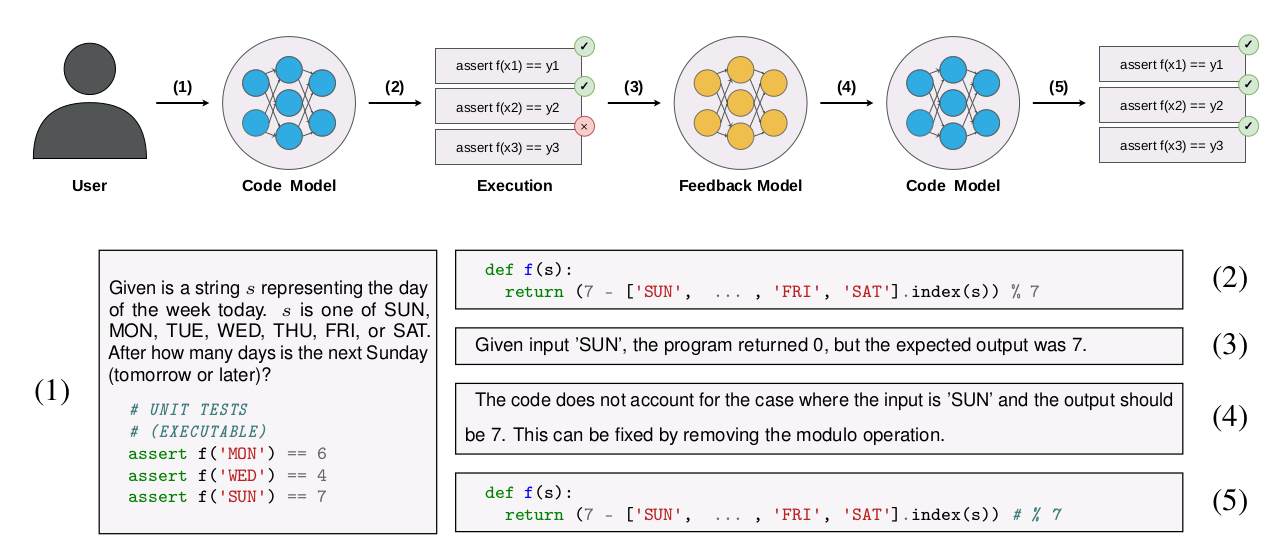
\includegraphics[scale=0.25]{png/example.png}
    \begin{itemize}
        \item  提出了一种完全由LLM + 启发式搜索算法结合的TOT算法,其可以从多条解决路径,快速的找到最佳解决方法,可以解决的一些复杂的,GPT-4都表现差的一些任务。其主要由thought生成、thought评估、搜索算法组成,可以生成解决方案、对方案进行自我评估、同时可以通过回溯算法来延续之前的解决思路,利用剪枝算法过滤不可靠解决方案,提升找到最优解决路径的速度。
        \item TOT其各个部分都是高度模块化的,例如可以用不同的LM,不同的搜索算法来实现,通用性比较强,同时其对于每个任务thought的定义都不太一致,如何针对不同的任务设置更好的thought也比较重要,他这里提出了“不能太小”、“不能太大”的指导原则可以参考。
        \item  LMs与经典人工智能方法的交叉是未来工作的一个重要的方向。
        % \item TOT直接利用LM的评估器效果还有待提高,Mini Crosswords results任务利用更好的state评估器,可能得到更大的提升,Game级别解决率从2\0%->35\%,说明利用更好的评估器也是非常重要的,可以取得更好的结果。
        % \item OpenAI的Andrej Karpathy在state of gpt中也提到了TOT算法,其也可能是比Auto-GPT更好的一种,让llm进行深思熟虑来解决复杂问题的一种实现思路。 
    \end{itemize}
\end{frame}



\begin{frame}
    \frametitle{相关启示}
    \begin{itemize}
        \item 针对我们目前做的时间序列的提示:可以参考他的思维分解,将我们的问题直接归到时间序列预测问题.
        \item 在思维产生的时候可以是对于我们当前序列的一些更正.想法可以是不同的拟合方式,也可以是的时间序列预测的相关方法,选择相应最合适的方法.然后通过相应的评估(比如计算MAE,MSE)作为最终的判别条件.
        % \item 遇到相应的问题:
        % \eee{
            % \item 对于每种拟合方式都要算一遍可能速度会比较慢.
        % }
    \end{itemize}

\end{frame}

% \subsection{论文2} 
% \begin{frame}
%     \frametitle{MEGABYTE的新方法}
%     \begin{itemize}
%         \item 摘要:该论文提出了一种名为MEGABYTE的新方法,用于对超过一百万字节的长序列进行建模。它使用多尺度解码器架构,将序列分成补丁,并在补丁中使用局部子模型,在补丁之间使用全局模型,从而实现次二次自我注意力,提高解码过程中的并行性。
%         \item 本文的贡献如下:
%         \eee{
%             \item 引入 MEGABYTE,这是一种使用多尺度解码器架构对长字节序列进行建模的新方法,该架构将序列分成补丁,在补丁中使用本地子模型,在补丁之间使用全局模型。en
%             \item 对 MEGABYTE 和强基线进行了广泛的实验,表明 MEGABYTE 允许字节级模型在长上下文语言建模中与子词模型竞争,在 ImageNet 上实现最先进的密度估计困惑,并允许从原始音频文件进行音频建模。n
%             \item 观察到,对于许多任务,大多数字节预测相对容易,这意味着没有必要按字节计算大型网络,并且可以使用小得多的模型进行补丁内建模。
%         }
%         \item introduction:该论文的介绍突显了音乐、图像或视频文件等各个领域中数百万字节的序列无处不在。但是,大型变压器解码器通常只使用数千个上下文令牌,这限制了可以应用它们的任务集。本文介绍了 MEGABYTE,这是一种使用多尺度解码器架构对长字节序列进行建模的新方法,该架构将序列分成补丁,在补丁中使用局部子模型,在补丁之间使用全局模型。这种方法可以实现亚二次的自我注意力,提高解码过程中的并行度,从而以更低的成本提高训练和生成性能。
%         \item method:该论文提出了一种名为MEGABYTE的新方法,该方法使用多尺度解码器架构对长字节序列进行建模,该架构将序列分成补丁,并在补丁中使用局部子模型,在补丁之间使用全局模型。这种方法可以实现亚二次的自我注意力,提高解码过程中的并行度,从而以更低的成本提高训练和生成性能。该论文还对MEGABYTE和强基线进行了广泛的实验,表明MEGABYTE允许字节级模型在长上下文语言建模中与子词模型竞争,在ImageNet上实现最先进的密度估计困惑,并允许从原始音频文件进行音频建模。此外,本文还讨论了使用语言模型在推理过程中用速度换取性能的几种技巧,包括滑动窗口和跨步推理。但是,这些方法仅在与先前发表的作品进行比较时使用。
%         \item result:该论文对MEGABYTE和强基线进行了广泛的实验,表明MEGABYTE允许字节级模型在长上下文语言建模中与子词模型竞争,在ImageNet上实现最先进的密度估计困惑,并允许从原始音频文件进行音频建模。本文还讨论了使用语言模型在推理过程中用速度换取性能的几种技巧,包括滑动窗口和跨步推理。但是,这些方法仅在与先前发表的作品进行比较时使用。
%         \item conclusion:该论文得出的结论是,拟议的多尺度解码器架构MEGABYTE是一种用于对长序列进行建模的可扩展方法,在一系列任务和模式中,它的性能优于现有的字节级模型,允许使用超过100万个令牌的大型序列。它还使用子词模型提供了具有竞争力的语言建模结果,这可能允许字节级模型取代标记化。但是,这里的实验规模远低于最先进的语言模型的规模,未来的工作应该探索将MEGABYTE扩展到更大的模型和数据集。
%     \end{itemize}
%     \eee{
%         \item 这个模型需要对transformer很了解才能看,还是就算了,不看这篇了.
%     }
% \end{frame}




% \subsection{论文3}
% \begin{frame}
%     \frametitle{大规模气象数据进行全面的天气预报}
%     \begin{itemize}
%         \item 摘要:论文摘要描述了需要一个协作平台,用于对大规模气象数据进行全面的天气预报。该论文提出了一种新颖的联邦学习方法,用于在具有异构气象数据的参与者中协作学习基于时空变压器的基础模型,以及一种满足资源匮乏传感器的通信和计算限制的即时学习机制。
%         \item 本文的贡献如下:
%         \eee{
%             \item 开发能够理解复杂的气象数据并提供跨区域天气预报的基础模型。 
%             \item 提出一种新颖的联邦学习方法,用于在具有异构气象数据的参与者中协作学习基于时空变压器的基础模型。 
%             \item 采用一种新颖的即时学习机制来满足资源匮乏传感器的通信和计算限制。 
%             \item 使用三个具有多变量时间序列的气象数据集,演示了拟议方法在经典天气预报任务中的有效性。
%         }
%         \item introduction:论文的导言强调了全球气候变化对不同区域的影响,以及需要一个大规模的协作数据共享平台来应对这一挑战。本文建议使用机器学习技术来提高解决这个问题的效率。但是,区域的异质性给采用集中统一模式为所有区域提供服务带来了挑战。
%         \item method:该论文提出了一种新颖的联邦学习方法,用于在具有异构气象数据的参与者中协作学习基于时空变压器的基础模型。所提出的方法使用一种新颖的即时学习机制来满足资源匮乏传感器的通信和计算限制。本文还介绍了一种空间即时学习(SPL)方法,该方法可以从空间角度在本地客户身上建立气象因素之间的相关性。使用三个具有多变量时间序列的气象数据集,证明了所提出的方法在经典天气预报任务中的有效性。
%         \item result:本文使用三个具有多变量时间序列的气象数据集,演示了所提出的方法在经典天气预报任务中的有效性。结果表明,所提出的方法在预测精度和效率方面优于最新方法。具体而言,所提出的方法显著提高了温度和降水的预测精度,而温度和降水是天气预报的关键因素。该论文还表明,该方法可以有效处理各地区气象数据的异质性,缓解数据暴露问题。
%         \item conclusion:该论文提出了一种新的机器学习方法来训练天气预报任务的基础模型,该方法能够捕捉基于多变量时间序列的气象数据的时空关系。本文在FL框架内引入了一种基于固定基础模型的即时学习机制,以提高性能,同时保持数据安全并减少通信开销。此外,该论文利用基于图的方法来减轻数据异质性对模型有效性的影响。使用三个具有多变量时间序列的气象数据集,证明了所提出的方法在经典天气预报任务中的有效性。本文得出结论,该方法在预测精度和效率方面优于最先进的方法,可以有效处理各地区气象数据的异质性,缓解数据暴露问题。
%     \end{itemize}
%     \eee{
%           \item 这篇文章意义也不是很大!!
% }
% \end{frame}



\section{代码调试}

\subsection{结果展示}

\begin{frame}
    \frametitle{ 新的提示在部分训练数据中出现乱码现象}  
	\begin{itemize}
		\item 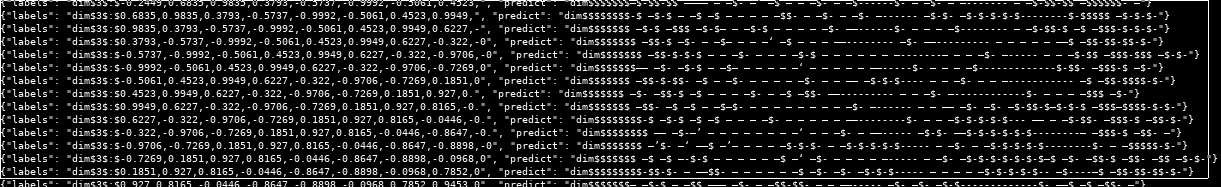
\includegraphics[scale=0.2555]{png/error1.png}
		\item 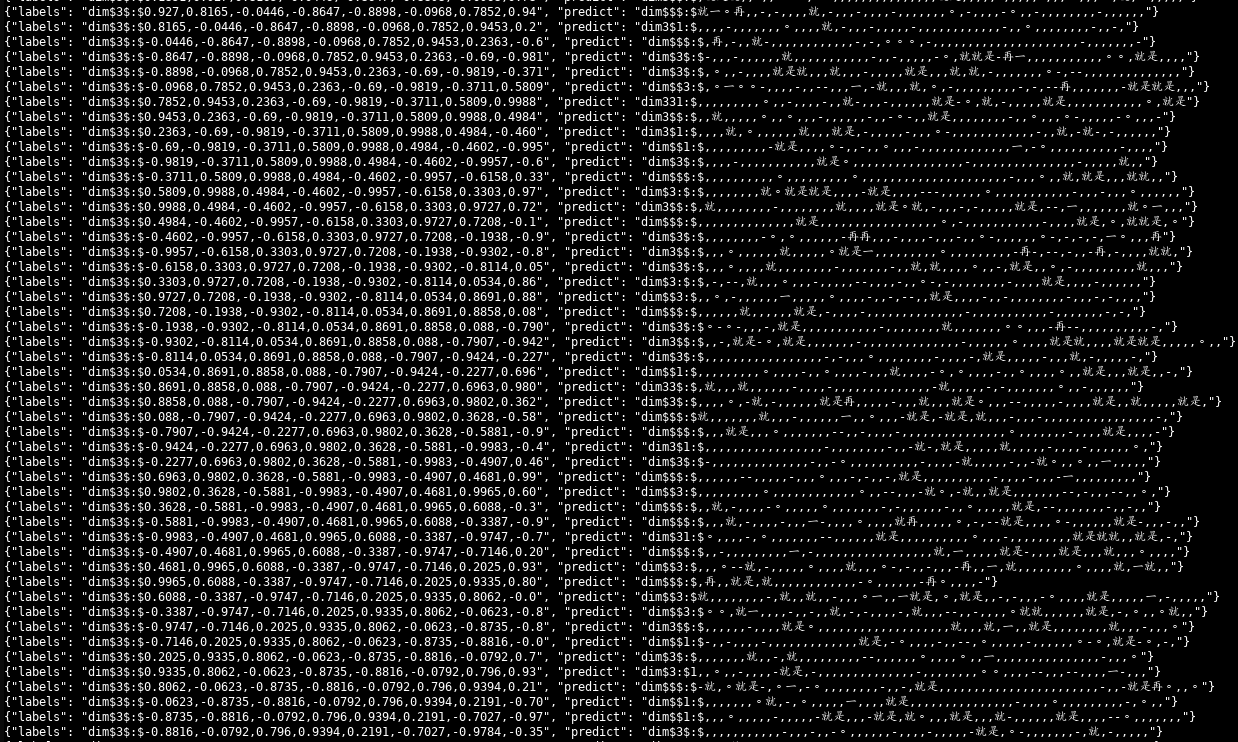
\includegraphics[scale=0.252]{png/error2.png}
	\end{itemize}
\end{frame}


\begin{frame}
    \frametitle{ new prompt(见过的任务)}  
	\begin{itemize}
		\item 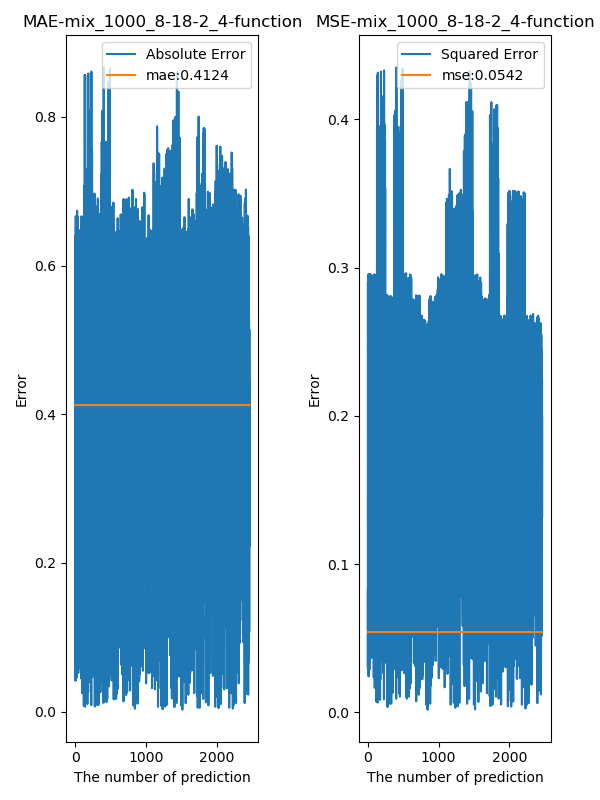
\includegraphics[scale=0.3555]{png/mix_1000_8-18-2_4-function.png}
        % \item 最终预测的所有结果都是长度为8的,但对于单一的任务是没有泛化能力的.
	\end{itemize}
\end{frame}

\begin{frame}
    \frametitle{ old prompt(见过的任务)}  
	\begin{itemize}
		\item 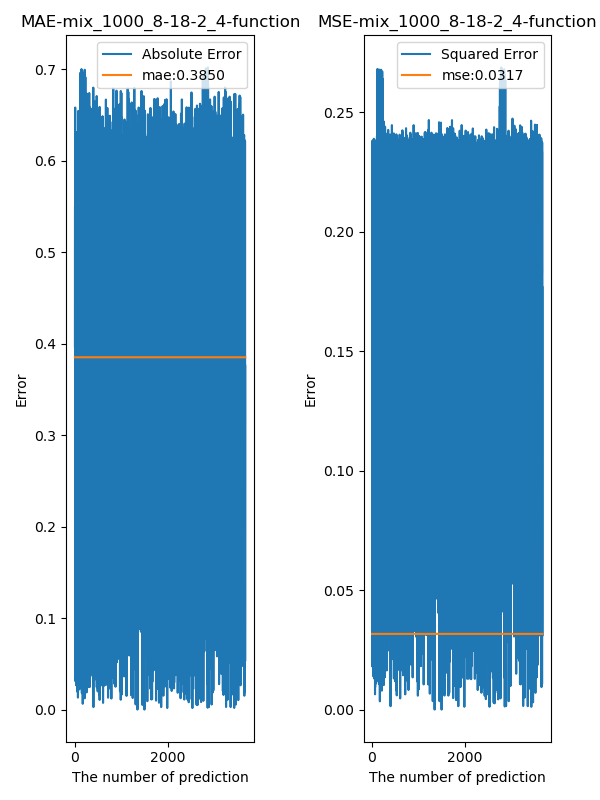
\includegraphics[scale=0.3555]{png/mix_1000_8-18-2_4-function_old-prompt.png}
	\end{itemize}
\end{frame}

\begin{frame}
    \frametitle{ new prompt(泛化性能测试)}  
	\begin{itemize}
		\item 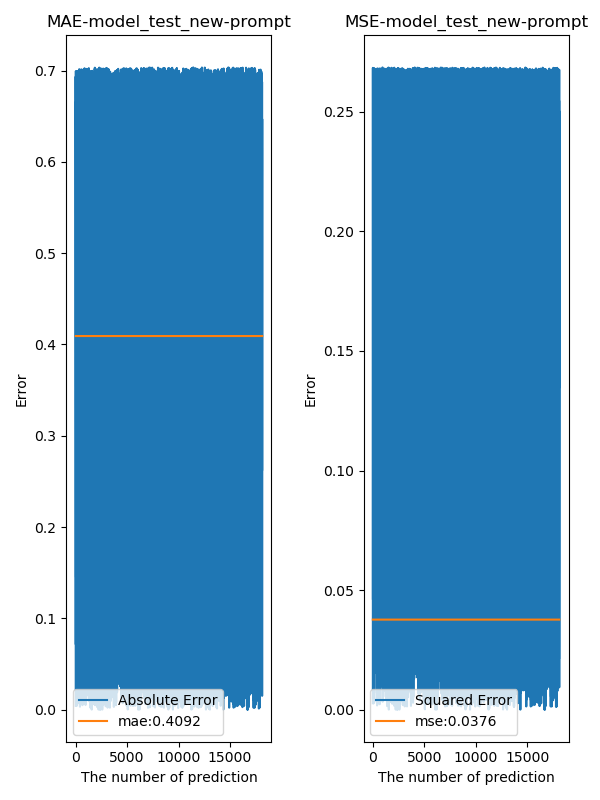
\includegraphics[scale=0.3555]{png/model_test_new-prompt.png}
	\end{itemize}
\end{frame}

\begin{frame}
    \frametitle{ old prompt(泛化性能测试)}  
	\begin{itemize}
		\item 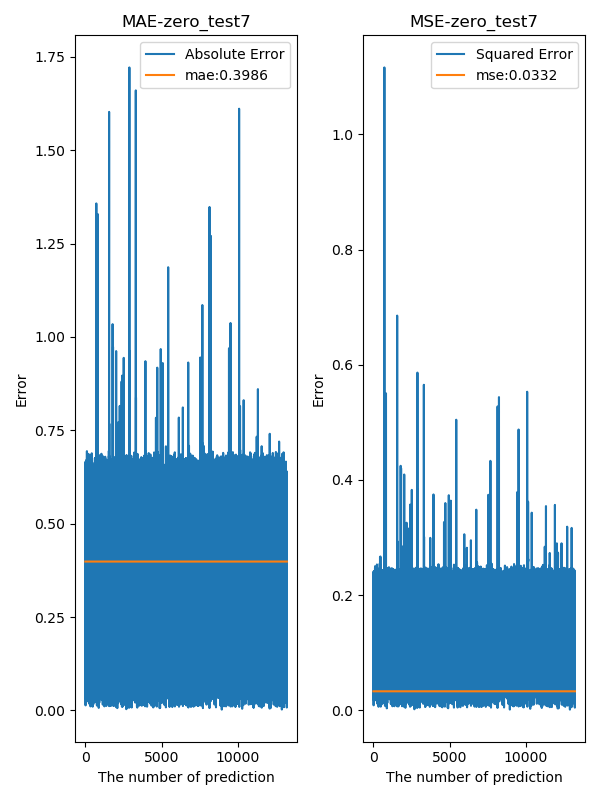
\includegraphics[scale=0.3555]{png/zero_test7.png}
	\end{itemize}
\end{frame}


% \begin{frame}
% 	% \frametitle{\tiny 准确率:66.95\%,使用具有zero\_model\_test去预测mix\_5000\_16-80-4\_2-function中的内容}
%     \frametitle{\tiny 训练总数据量:640000,预测长度:8预测4,...,80预测40,间隔4;用于训练的函数序列:8种基本函数,如三角,多项式函数,对数,平方根等 \\
%     待预测的数据:16预测8,...,80预测40,间隔为4;预测的函数序列:2种不同的函数序列;准确率:66.95\%} 
%     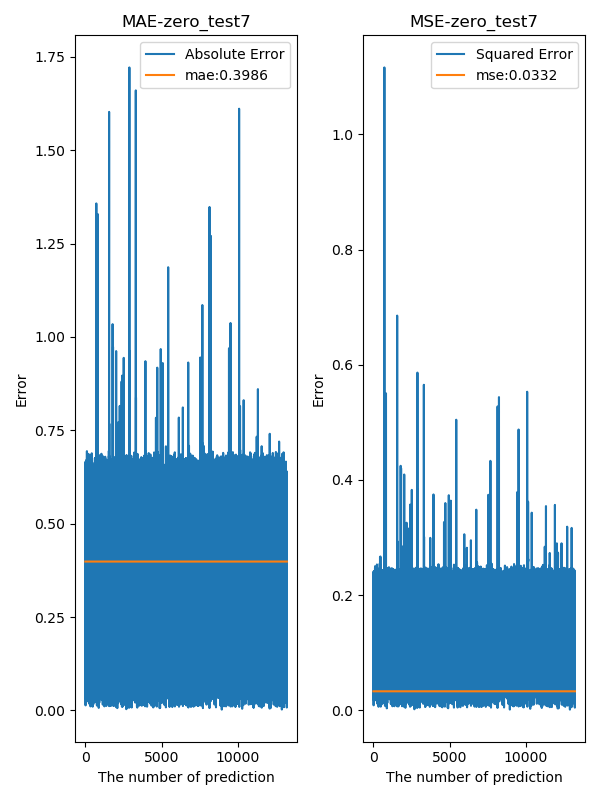
\includegraphics[scale=0.3555]{png/zero_test7.png}
% 	% \begin{itemize}
% 		%	\item 是否一个更加综合的模型能够对结果有更强的泛化能力?
% 	% \end{itemize}
% \end{frame}


% \begin{frame}
% 	\frametitle{\small 总数据量:30000,16预测8,长向量序列预测}	
% 	\begin{itemize}
% 		% \item 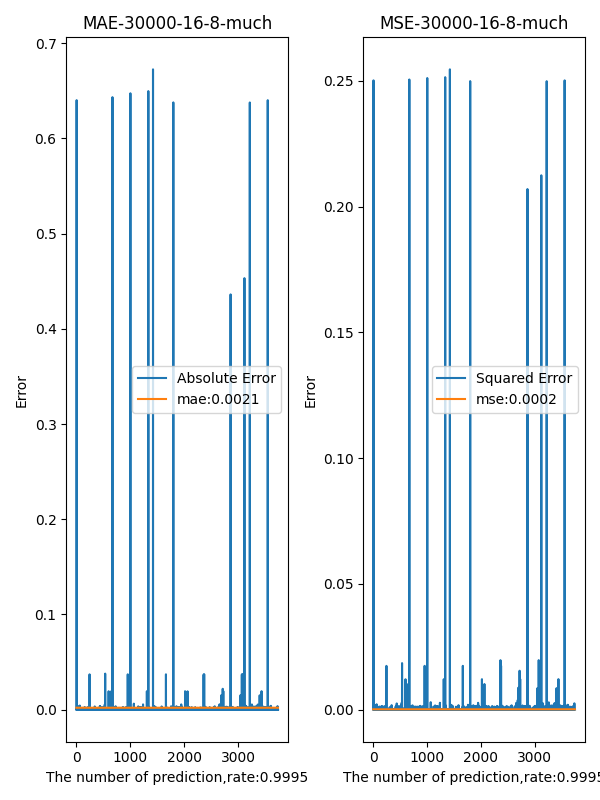
\includegraphics[scale=0.3555]{png/30000-16-8-much.png}
% 	\end{itemize}
% \end{frame}

\subsection{实验结果分析}
\begin{frame}
	\frametitle{实验结论}	
	\begin{itemize}
        \item 新的提示和旧的提示在没见过的任务上的性能上的测试以及在见过的任务上的测试基本一致,甚至旧的提示比新提示效果更好!从中可以看出修改提示的排列可能对模型最终的训练影响不大.
        \item 使用新的提示后,部分测试结果出现了乱码现象.
        \eee{
            \item 使用chatglm2训练一个大型数据集合时,在预测已经见过的任务上出现了乱码的现象.
            \item 使用chatglm进行泛化测试的一个实验,也出现了乱码的情况.
        }
	\end{itemize}
\end{frame}

% \subsection{实验过程中遇到的一些问题}

% \begin{frame}
% 	\frametitle{遇到的问题}	
% 	\begin{itemize}
%         \item 目标预测的个数和实际预测个数不同或者预测非数值形式,下面是一些解决方法
%         \eee{
%             \item 忽略实际预测个数和目标个数不同的例子,并计算其比率rate(目标与实际个数相同的个数/测试集个数)
%             \item 对预测得到的结果进行截断或补零
%         }   
%         \item 序列长度太长的问题
% 	\end{itemize}
%     % 目前考虑的是只考虑数量对等的
% \end{frame}


\subsection{下一步的计划}
\begin{frame}
	\frametitle{下一步计划}	
	\begin{itemize}
        % \item 混合更多的元素,同时训练更多不同种类的时间序列和以及预测长度。
        % \item 尝试对未见过的序列进行预测,看看结果如何。
        \item 是否还要使用新的提示方式?(可能更加简洁的提示效果会更好)
        \item 如何提高模型的泛化能力
        \eee{
            \item 在通过修改提示的方式上目前效果不太好.
            % \item 使用数据增强操作.
            \item 通过迁移学习来提高泛化能力.
            \item 寻找提高模型泛化能力的相关论文?
        }
        \item 进行时间序列的预测.
        % 开始做一些对比实验吧.同步前进.
	\end{itemize}
\end{frame}

% 结束语
\section{}
\begin{frame}
	\frametitle{}
	\begin{center}
		\Huge{谢谢老师和同学们的聆听!}
	\end{center}
\end{frame}

\end{CJK*}
\end{document}